% !TeX spellcheck = cs_CZ
%{\tikzset{external/prefix={tikz/FYZI/}}
% \tikzset{external/figure name/.add={ch03_}{}}
%---------------------------------------------------------------------------------------------------
% file fey1ch05.tex
%---------------------------------------------------------------------------------------------------
%================= Kapitola: Čas a vzdálenost =====================================================
\setchaptertoc
\chapter{Čas a vzdálenost}\label{chap:fey_cas}

  \section{Pohyb}
    V této kapitole si všimneme některých představ o čase a vzdálenosti Již jsme zdůraznili, že 
    fyzika - právě tak jako další vědy - závisí na pozorování. Je možné říci, že vývoj fyzikálních 
    věd do jejich dnešní podoby závisel do značné míry na důrazu, který se kladl na kvantitativní 
    pozorování. Jen pomocí kvantitativních pozorování je možné dospět ke kvantitativním vztahům, 
    jež jsou srdcem fyziky.
    
    Podle názoru mnohých se začátky fyziky datují od výzkumů Galileových před 350 lety, a Galileo 
    je vlastně považován za prvního fyzika. Do té doby mělo studium pohybu jen filozofický 
    charakter a spočívalo na argumentech, k nimž bylo možno dospět pouhým uvažováním. Většina 
    argumentů pocházela od Aristotela a jiných řeckých filozofů a tyto argumenty byly považovány za 
    \uv{dokázané}. Galileo však byl v tomto směru skeptický a pustil se do následujícího 
    experimentu při zkoumání pohybu: Nechal kuličku koulet po nakloněné rovině a pozoroval pohyb. 
    Nejen že se díval, ale i měřil, jak daleko kulička za jaký čas dojde.
    
    \luagraphic[0.7]{fyz_fig064.pdf}{Zatížená tyč podepřená na jednom konci 
    (\cite[s.~64]{Feynman01})}{fyz:fig064}
    
    Způsob měření vzdálenosti byl dobře znám dávno před Galileem, neexistovaly však přesné způsoby 
    měření času, zejména krátkých časů. Ačkoli sám později vynalezl spolehlivější hodiny (ne však 
    takové, jaké známe dnes), prováděl Galileo své první experimenty tak, že pomocí vlastního 
    pulzu určoval stejné časové intervaly. Udělejme nyní totéž:
    
    Počítejme údery tepu po dobu pohybu kuličky: „raz... dva... tři... čtyři... pět... šest... 
    sedm... osm...“. Požádejme kolegu, aby označil polohu kuličky při každém tepu. Tak můžeme 
    \emph{změřit vzdálenost}, kterou kulička urazila od vypuštění za jeden, dva, tři atd. stejné 
    intervaly času. Galileo vyjádřil výsledek svých pozorování následujícím způsobem: Když si 
    polohu kuličky značíme po \num{1}, \num{2}, \num{3}, \num{4} ... jednotkách času od jejího 
    vypuštění, pak jsou tyto značky vzdáleny od počátečního bodu úměrně číslům \num{1}, \num{4}, 
    \num{9}, \num{16} ... Dnes bychom řekli, že vzdálenost je úměrná druhé mocnině času
    \begin{equation*}
      s \sim t^2.
    \end{equation*}
    
    Studium \emph{pohybu}, které je základem všech fyzikálních disciplín, se zabývá dvěma otázkami: 
    kde? a kdy?
    
  \section{Čas}
    Nejprve se zamysleme nad tím, co chápeme jako \emph{čas}. Co \emph{je} čas? Bylo by krásné, 
    kdyby se nám podařilo najít dobrou definici času. Ve slovnících nacházíme „čas“ definovaný jako 
    „období“ a „období“ zase jako „čas“, což se nezdá být příliš použitelné. Snad bychom mohli 
    říci: „Čas je to, co se děje, když se nic jiného neděje.“ To nás však nedovede příliš daleko. 
    Je snad právě tak dobré, když si přiznáme, že čas je jedna z těch věcí, kterou pravděpodobně 
    nemůžeme definovat (v slovníkovém smyslu), a říkat o něm jen to, co už víme: Čas je to, jak 
    dlouho čekáme!
    
    Skutečně důležité však není to, jak čas \emph{definujeme}, ale jak ho \emph{měříme}. Jedním ze 
    způsobů měření časuje využití něčeho, co se neustále děje, a to pravidelným způsobem - něčeho, 
    co je \emph{periodické}. Například den. Den, ten se stále opakuje. Když však o tom uvažujeme, 
    můžeme si položit otázku: .Jsou dny periodické, jsou pravidelné? Mají všechny dny stejnou 
    délku?“ Určitě máme dojem, že letní dny jsou delší než zimní. Ovšem, když se moc nudíme, 
    připadají nám i některé zimní dny velmi dlouhé. Již jsme určitě slyšeli někoho zvolat: „Ach, to 
    byl dnes dlouhý den!“
    
    Zdá se však, že dny jsou v \emph{průměru} téměř stejně dlouhé. Existuje způsob, jak prověřit, 
    jsou-li dny stejně dlouhé, buď dva za sebou následující nebo alespoň v průměru? Jedním ze 
    způsobů je porovnání s jiným periodickým jevem. Všimněme si, jak je možné takové porovnání 
    provést pomocí přesýpacích hodin. Pomocí přesýpacích hodin „vytvoříme“ periodičnost, budeme-li 
    je ve dne v noci překlápět, jakmile se přesype poslední zrnko písku.
    
    Potom nám stačí spočítat počet překlopení hodin od jednoho do druhého rána. Tak zjistíme, že 
    počet „hodin“, tj. překlopení, není každý „den“ stejný! Mohli bychom podezřívat Slunce nebo 
    přesýpací hodiny nebo oboje. Po jistých úvahách by nás mohlo napadnout, že „hodiny“ je třeba 
    počítat od poledne do poledne. (Poledne tu \emph{nedefinujeme} jako 12.00 hodin, ale jako 
    okamžik, kdy Slunce vrcholí.) Tentokrát bychom zjistili, že každý den má stejný počet „hodin“. 
    Získali jsme jakousi důvěru, že jak „hodina“, tak „den“ se pravidelně opakují, tj. vyznačují po 
    sobě následující stejné časové intervaly, ačkoli jsme \emph{nedokázali}, že jsou „skutečně“ 
    periodické. Je možné si položit otázku, zda by nemohla jakási zázračná bytost zpomalovat pohyb 
    písku v noci a urychlovat ho ve dne. Náš experiment na takovouto otázku odpověď nedává. Můžeme 
    říci jen tolik, že jsme zjistili, že pravidelnost jednoho druhu je ve shodě s pravidelností 
    jiného druhu. Můžeme říci, že naše definice času spočívá v opakování se určité zřejmě  
    periodické události.
    
  \section{Krátké časy}
    Měli bychom si uvědomit, že při zkoušce opakování dne jsme získali i další důležitý poznatek. 
    Našli jsme způsob přesnějšího měření \emph{částí} dne. Našli jsme způsob měření kratších 
    časových úseků. Můžeme v tomto postupu pokračovat a tak měřit ještě kratší časové intervaly?
    Galileo zjistil, že kyvadlo vykoná každý kyv za stejnou dobu, zůstává-li velikost rozkyvu malá. 
    Potvrzuje to test určující počet kyvů kyvadla za jednu „hodinu“. Takto můžeme vytvořit značky 
    zlomků hodiny. Použijeme-li mechanické zařízení na počítání kyvů a na udržení chodu kyvadla - 
    získáme kyvadlové hodiny našich dědečků.
    
    Dohodněme se, že jestliže naše kyvadlo kmitá \num{3600}-krát za hodinu (a je-li takových hodin
    \num{24} za den), nazveme periodu kyvadla jednou „sekundou“. Tak jsme naši původní časovou
    jednotku rozdělili přibližně na \num{10e5} částí. Stejně můžeme sekundu rozdělit na menší a
    menší intervaly. Zjistíme, že není praktické konstruovat mechanická kyvadla, která kývají
    libovolně rychle, ale můžeme konstruovat \emph{elektrická} kyvadla, nazývaná
    \textbf{oscilátory}, která nám poskytnou periodicitu s velmi krátkými periodami kmitů. V
    takových elektronických oscilátorech je to elektrický proud, který kmitá podobným způsobem jako
    kyvadlo.
    
    Můžeme sestrojit celou řadu takových elektronických oscilátorů, každý s periodou desetkrát
    kratší, než má předcházející. Každý oscilátor můžeme „kalibrovat“ vůči sousednímu pomalejšímu
    oscilátoru určením počtu kmitů,jež vykoná za dobu jednoho kmitu pomalejšího oscilátoru. Je-li
    perioda kmitů našich hodin kratší než zlomek sekundy, nemůžeme určovat kmity bez pomocného
    zařízení, které rozšiřuje naši pozorovací schopnost. Jedním z takových zařízení je
    \emph{osciloskop} s elektronovým paprskem, jenž pracuje jako jakýsi mikroskop pro krátké časy.
    Toto zařízení zakresluje na fluorescenční stínítko graf elektrického proudu (nebo napětí) v
    závislosti na čase. Připojíme-li osciloskop ke dvěma sousedním oscilátorům z naší posloupnosti
    tak, že nejprve zakresluje proud jednoho a potom proud druhého oscilátoru, dostáváme dva grafy
    podobné těm, které jsou znázorněny na obr. \ref{fyz:fig065}. Tak můžeme pohotově určit počet
    period rychlejšího oscilátoru po dobu jedné periody pomalejšího oscilátoru. 
    
    \begin{figure}[ht!]  %\ref{fyz:fig065}
      \centering
      \subcaptionbox{\label{fyz:fig065a}}{\luafigure[0.4]{fyz_fig065a.png}} \hspace{2em}
      \subcaptionbox{\label{fyz:fig065b}}{\luafigure[0.4]{fyz_fig065b.png}}
      \caption{Dva pohledy na obrazovku osciloskopu: a) osciloskop je připojen k jednomu oscilátoru.
               b) osciloskop je připojen k oscilátoru, jehož perioda je desetinou periody 
               předcházejí oscilátoru (\cite[s.~66]{Feynman01})}
      \label{fyz:fig065}
    \end{figure}
    
    Pomocí moderních elektronických metod byly zkonstruovány oscilátory s periodou krátkou kolem 
    \num{10e-12} sekund a byly kalibrovány (porovnávacími metodami podobnými metodě, kterou
    jsme popsali) v naší standardní časové jednotce - sekundě. Vynalezení a zdokonalení „laseru“ 
    neboli zesilovače světla umožnilo v nedávných letech konstrukci oscilátorů s ještě kratšími 
    periodami než \num{10e-12} sekundy, ale zatím je nebylo možné kalibrovat popsaným způsobem, 
    ačkoli i k tomu nepochybně dojde.
    
    Časy kratší než \num{10e-12} sekundy byly měřeny, ale jinými způsoby. Ve skutečnosti byla 
    použita jiná \emph{definice} „času“. Jedním ze způsobů bylo pozorování mezi dvěma událostmi, 
    jež se stanou s pohybujícím se předmětem. Jestliže například zapneme a pak vypneme reflektory 
    pohybujícího se auta, můžeme určit, jak \emph{dlouho} byla světla zapnutá, jestliže víme, 
    \emph{kde} byla zapnuta a vypnuta a jakou rychlostí se auto pohybovalo. Čas určíme tak, že 
    vzdálenost, po kterou byla světla zapnutá, dělíme rychlostí.
    
    Nedávno byla taková metoda použita pro měření doby života \(\pi^0\) mezonu. Mikroskopickým 
    pozorováním drobných stop zanechaných ve fotografické emulzi, v níž byl mezon vytvořen, se 
    zjistilo, že \(\pi^0\) mezon (pohybující se rychlostí téměř rovnou rychlostí světla) urazil v 
    průměru vzdálenost \num{10e-7} metrů dříve, než se rozpadl. Žil jen přibližně \num{10e-16} 
    sekundy. Je třeba však zdůraznit, že jsme použili trochu jinou definici „času“ než předtím. 
    Dokud však není rozpor v našem chápání, věříme, že tyto definice jsou dostatečně rovnocenné.
    
    Dalším rozšířením našich metod - a je-li to nevyhnutelné i našich definicí - můžeme určit 
    trvání ještě rychlejších fyzikálních jevů. Můžeme hovořit o periodě jaderných kmitů. Můžeme 
    hovořit o délce života nově objevených podivných rezonancí (částic). Jejich celková délka 
    života je pouze \num{10e-24} sekundy, což je přibližně doba, kterou potřebuje světlo 
    (pohybující se největší ze známých rychlostí) k průchodu jádrem vodíku (což je 
    nejmenší známý předmět).
    
    Co je možné říci o ještě kratších časech? Existuje čas v ještě menším měřítku? Má vůbec smysl 
    hovořit o ještě kratších časech, když neumíme měřit - nebo dokonce si rozumně představit - 
    něco, co se odehrává v kratším čase? Snad ne. Toto jsou některé otevřené otázky, které si 
    budeme klást a na které snad nalezneme odpověď za dalších dvacet nebo třicet let.
    
  \section{Dlouhé časy}
    Nyní uvažujme časy delší než jeden den. Měření dlouhých časů je jednoduché; budeme prostě 
    počítat dny - dokud bude existovat někdo, kdo to bude moci dělat. Tak docházíme k další 
    přirozené periodicitě: roku, který má přibližně \num{365} dní. Zjišťujeme i to, příroda nám 
    někdy poskytuje počítadlo let, a to v podobě letokruhů stromů nebo říčních naplavenin. V 
    některých případech můžeme využít těchto přírodních časových značek k určení času, který 
    uplynul od nějaké dávné události.
    
    Nemůžeme-li při měření dlouhých časů počítat roky, musíme hledat jiný způsob měření. Jedním z 
    nejúspěšnějších je použití \emph{radioaktivního materiálu} jako „hodin“. V tomto případě nemáme 
    periodický proces tak jako v případě dne nebo kyvadla, ale máme nový druh „pravidelností“. 
    Zjišťujeme, že radioaktivita jistého vzorku materiálu klesá o stejné \emph{procento},    
    jestliže ji určujeme ve dvou stejných po sobě jdoucích přírůstcích jeho věku. Nakreslíme-li 
    graf radioaktivity v závislostí na čase (měřeného např. ve dnech), dostaneme křivku jako na 
    obr. \ref{fyz:fig066}. Vidíme, že v případě poklesu radioaktivity na jednu polovinu za \(T\) 
    dní (\(T\) nazýváme „poločasem rozpadu“) dochází k poklesu na jednu čtvrtinu za dalších \(T\) 
    dní atd. V libovolném časovém intervalu \(t\) je obsaženo \(t/T\) „poločasů rozpadu“ a podíl 
    aktivity, která zbývá po čase \(t\) je roven \((l/2)^{\frac{t}{T}}\).

    \begin{figure}[ht!]  %\ref{fyz:fig066}
      \centering
      \luafigure[0.6]{fyz_fig066.pdf}
      \caption{Pokles radioaktivity s časem; aktivita klesne o polovinu za dobu \uv{poločasu 
               rozpadu} (\cite[s.~68]{Feynman01})}
      \label{fyz:fig066}
    \end{figure}    
    Víme-li, že kousek materiálu, například dřeva, obsahoval při svém vzniku množství \(A\) 
    radioaktivního materiálu a přímým měřením zjistíme, že nyní obsahuje množství \(B\), můžeme 
    vypočítat věk předmětu \(t\) řešením rovnice
    \begin{equation}\label{fyz:eq065}
      \left(\dfrac{1}{2}\right)^{\dfrac{t}{T}} = \dfrac{B}{A}
    \end{equation}
    
    Naštěstí existují případy, v nichž známe množství radioaktivity přítomné při vzniku předmětu. 
    Víme například, že oxid uhličitý ve vzduchu obsahuje malý zlomek radioaktivního izotopu uhlíku 
    \ce{^{14}C} (neustále doplňovaný působením kosmického záření). Když měříme \emph{celkový} obsah 
    uhlíku v předmětu, víme, že určitý zlomek tohoto množství byl původně radioaktivní \ce{^{14}C}, 
    a proto známe počáteční množství \(A\) vystupující v uvedeném vztahu. Uhlík \ce{^{14}C} má 
    poločas rozpadu \num{5000} let. Pečlivým měřením můžeme zjistit množství, které zůstalo po 
    \num{20} poločasech rozpadu nebo jiném podobném čase a můžeme proto stanovit stáří předmětů z 
    organických látek, které rostly už před \num{100000} lety.
    
    Zajímá nás však i věk ještě starších věcí a zdá se, že ho umíme určit. Mnohé z našich poznatků 
    jsou založeny na měření jiných radioaktivních izotopů, jež mají různé poločasy rozpadu. 
    Použijeme-li izotop, jenž má delší poločas rozpadu, můžeme měřit delší časy. Například uran má 
    izotop, jehož poločas rozpadu je asi \num{10e9} let, takže když nějaký materiál při svém 
    vytvoření před \num{10e9} lety obsahoval uran, zůstane dnes z tohoto uranu jen polovina. Uran 
    se při rozpadu mění na olovo. Uvažujme kousek horniny, jenž vznikl před mnoha lety nějakým 
    chemickým procesem. Olovo, jež se chemicky liší od uranu, by mělo být v jedné části horniny a 
    uran v jiné části horniny. Uran a olovo jsou tedy při vzniku horniny odděleny. Jestliže však 
    tentýž kousek horniny zkoumáme dnes, pak na místě, kde byl původně uran, najdeme určitou část 
    uranu a určitou část olova. Porovnáním těchto částí můžeme určit, kolik procent uranu zaniklo a 
    přeměnilo se na olovo. Touto metodou bylo stáří některých hornin určeno na několik miliard let. 
    Zobecněním této metody, kdy místo v horninách byly uran a olovo sledovány v mořích a byly 
    uvažovány celosvětové průměry, se podařilo (v průběhu nedávných let) určit stáří Země na 
    přibližně \num{5.5} miliardy let.
    
    Povzbuzující je zjištění, že podle uranové metody je Země stejně stará jako meteority, které na 
    ni dopadají. Vypadá to tedy tak, že Země byla vytvořena z kusů skal létajících prostorem a 
    meteority jsou pravděpodobně zbytky tohoto materiálu. Někdy před více než pěti miliardami let 
    měl vesmír svůj počátek. Dnes se domníváme, že alespoň část vesmíru měla počátek před deseti 
    nebo dvanácti miliardami let. Nevíme, co se stalo předtím. Mohli bychom se vlastně ptát: „Má 
    taková otázka smysl? Má dávno minulý čas vůbec nějaký smysl?“
    
    \begin{figure}[ht!]  %\ref{fyz:fig075}
      \centering
      \luafigure[1]{fyz_fig075.pdf}
      \caption{Tabulka časů (\cite[s.~69]{Feynman01})}
      \label{fyz:fig075}
    \end{figure}

  \section{Jednotky a standardy času}
    Již jsme naznačili, že je vhodné vycházet z nějaké standardní časové jednotky a ostatní časy 
    vztahovat k jejím násobkům nebo zlomkům. Co máme vzít jako základní standard času? Máme za něho 
    zvolit tep lidského srdce? Porovnáme-li tepy, zjistíme, že se značně liší. Porovnáním dvou 
    hodin zjistíme, že se jejich údaje tak mnoho neliší. Proto by bylo možné vzít za standard 
    hodiny. Jenže čí hodiny. Existuje pohádka o švýcarském chlapci, který chtěl, aby všechny hodiny 
    v jeho městě zvonily poledne ve stejnou chvíli. Tak se vydal na cestu, aby přesvědčil lidi o 
    užitečnosti této myšlenky. Každý vlastník hodin považoval tuto myšlenku za vynikající, ale jen 
    v případě, kdy by se všechny ostatní hodiny přizpůsobily jeho hodinám. Je dost těžké 
    rozhodnout, které hodiny je třeba vzít za standard. Naštěstí všichni uznáváme jedny hodiny - 
    Zemi. Perioda otáčení Země byla dlouho považována za časový standard. Když však byla měření 
    stále přesnější, zjistilo se, že rotace Země není dokonale periodická, měříme-li ji 
    nejpřesnějšími hodinami. Těmi „nejpřesnějšími“ hodinami jsou ty, jejichž přesnosti důvěřujeme 
    proto, že jejich údaje navzájem souhlasí. Dnes víme, že z různých důvodů jsou některé dny 
    kratší, jiné delší a v průměru se s postupem času perioda otáčení Země trochu prodlužuje.
    
    Až donedávna jsme nenašli nic lepšího, než periodu zemské rotace, takže všechny hodiny se 
    vztahovaly k délce dne a sekunda byla definována jako \(\frac{1}{\num{86400}}\) středního 
    slunečního dne. Nedávno jsme však získali zkušenosti s některými přírodními oscilátory, o nichž 
    dnes předpokládáme, že poskytují stálejší časový normál než Země a jsou také založeny na 
    přírodním jevu přístupném všem. Jsou to tzv. „atomové hodiny“. Jejich základní vnitřní periodou 
    je perioda atomových kmitů, jež téměř nezávisí na teplotě a jiných vnějších vlivech. Tyto 
    hodiny měří čas s přesností lepší než \num{10e-9}.
    
    Protože se podařilo sestrojit hodiny, udávající čas mnohem přesněji než astronomické metody, 
    je dnes sekunda definována Jako doba trvání \num{9192631770} period záření, které odpovídá 
    přechodu mezí dvěma hladinami velmi jemné struktury základního stavu atomu cesia \num{133}.
    
    %--Slunce vleže na břehu klidného moře--------------------------
    % !TeX spellcheck = cs_CZ
\begin{fyzexam}{Představme si, že pozorujeme západ Slunce vleže na břehu klidného moře. Spustíme
  stopky právě v okamžiku, kdy Slunce zcela zmizí. Poté vstaneme a zvýšíme tak polohu svých očí o
  \SI{1.70}{\m}. Stopky zastavíme v okamžiku, kdy nám Slunce zmizí podruhé. Jaký je poloměr Země,
  ukazují-li stopky \SI{11.1}{\s}?}{exam014}

  {\centering
   \captionsetup{type=figure}
   \luafigure[1]{fyz_fig885.jpg}
   \captionof{figure}{Opravdu je možné změřit Zemi tak prostým pozorováním}
   \label{fyz:fig885}
   \par
  }

  Z obr. \ref{fyz:fig884} vidíme, že při pozorování vleže se zorný paprsek směřující k hornímu
  okraji slunečního kotouče dotýká povrchu Země v místě, ve kterém se právě nacházíme, tj. v bodě
  \(A\). Při druhém pozorování západu Slunce je zorný paprsek tečnou v bodě \(B\). Označme symbolem
  \(d\) vzdálenost mezi bodem \(B\) a polohou očí stojícího pozorovatele. Vzdálenosti bodů \(A\) a
  \(B\) od středu Země jsou rovny poloměru Země \(r\). Z Pythagorovy věty dostaneme
  \begin{equation*}
    d^2 + r^2 = (r + h)^2 = r^2 + 2rh + h^2\;\Rightarrow\; d^2 = 2rh + h^2.
  \end{equation*}

  Výška \(h\) je ovšem zanedbatelná vzhledem k poloměru Země \(r\). Proto je člen \(h^2\) mnohem
  menší než člen \(2rh\) a rovnici lze přepsat ve tvaru
  \begin{equation}\label{fyz:eq573}
    d^2 = 2rh
  \end{equation}

  Symbolem \(\varTheta\) jsme označili úhel mezi tečnami v bodech \(A\) a \(B\) (obr.
  \ref{fyz:fig884}). O stejný úhel se za změřenou dobu \SI{11.1}{\s} otočí Slunce na své zdánlivé
  dráze kolem Země. Za celý den, tj. přibližně za \num{24} hodin, se Slunce kolem Země otočí o
  \ang{360}. Pak můžeme psát
  \begin{equation*}
    \dfrac{\varTheta}{\ang{360}} = \dfrac{t}{\SI{24}{\hour}}.
  \end{equation*}
  Dosadíme-li \(t = \SI{11.1}{\s}\), dostaneme
  \begin{equation*}
    \varTheta = \dfrac{\ang{360}\cdot\SI{11.1}{\s}}
                      {\SI{24}{\hour}\cdot\SI{60}{\minute\per\hour}\cdot\SI{60}{\s\per\minute}}
              =\ang{0.04625}.
  \end{equation*}
  Z obr. \ref{fyz:fig884} vidíme, že \(d = r\cdot\tan{\varTheta}\). Dosazením do rov.
  (\ref{fyz:eq573}) dostaneme
  \begin{equation}\label{fyz:eq574}
    r^2\cdot\tan^2{\varTheta} = 2rh\quad\Rightarrow\quad 
    r = \dfrac{2h}{\tan^2{\varTheta}}.
  \end{equation}

  {\centering
  \captionsetup{type=figure}
  \luafigure[1]{fyz_fig884.pdf}
  \captionof{figure}{Zvedne-li se pozorovatel z polohy vleže (bod \(A\)) a zvýší tak polohu svých
    očí do výšky \(h\), otočí se zorný paprsek vycházející z horního okraje slunečního kotouče o
    úhel \(\varTheta\). (Velikosti výšky \(h\) i úhlu \(\varTheta\) jsou v obrázku mnohem větší, než
    odpovídá skutečnosti.)
  \cite[s.~229]{Halliday2001}
  \label{fyz:fig884}} \par}
  \vspace{1em}
  Pro číselné hodnoty \(\varTheta = \ang{0.04625}\) a \(h = \SI{1.70}{\m}\) máme konečně
  \begin{align*}
    r\cdot\tan{\varTheta} &= 2rh\quad\Rightarrow   \\
                        r &= \dfrac{2\cdot\SI{1.70}{\m}}{\tan^2{\ang{0.04625}}}=\SI{5.22e6}{\m}.
  \end{align*}
  Tento výsledek se liší od známé hodnoty poloměru Země (\SI{6.378e6}{\m}) o \SI{20}{\percent}.
\end{fyzexam}
    %---------------------------------------------------------------

  \section{Velké vzdálenosti}
    Nyní věnujme pozornost otázce \emph{vzdáleností}. Jak vzdálené, nebo jak velké jsou věci? Každý 
    ví, že při měření vzdáleností vezmeme tyč, postupně ji přikládáme a počítáme. Nebo si pomůžeme 
    palcem a počítáme. Začneme tedy s jednotkou a počítáme. Jak se však měří menší věci? Jak 
    rozdělujeme vzdálenosti? Stejně tak jako jsme rozdělovali čas: Vezmeme menší jednotku a 
    počítáme, kolik takových jednotek vytvoří větší jednotku. Tak můžeme měřit menší a ještě menší 
    délky.

    \begin{figure}[ht!]  %\ref{fyz:fig068}
      \centering
      \luafigure[0.9]{fyz_fig068.pdf}
      \caption{Výška družice určená triangulací (\cite[s.~70]{Feynman01})}
      \label{fyz:fig068}
    \end{figure}
    
    Vzdáleností však nerozumíme vždy to, co můžeme měřit metrovou tyčí. Bylo by těžké měřit 
    horizontální vzdálenost mezi dvěma vrcholy hor jen pomocí dřevěného metru. Ze zkušeností víme, 
    že vzdálenost je možné měřit i jiným způsobem - \textbf{triangulací}. To sice znamená použít 
    jinou definici vzdálenosti, ale v případech, kdy jsou obě dvě definice použitelné, dávají 
    shodný výsledek. Prostor je více méně tím, za co ho považoval Euklides, a proto jsou uvedené 
    definice shodné. Protože jsou shodné na Zemi, máme k triangulaci určitou důvěru i při použití 
    pro ještě větší vzdálenosti. Například pomocí triangulace jsme mohli změřit výšku první umělé 
    družice. Zjistili jsme, že byla asi \num{5e5} metrů vysoko. Při pečlivém měření můžeme podobně 
    změřit vzdálenost k Měsíci. Dva teleskopy na různých místech Země nám poskytnou dva úhly, které 
    potřebujeme. Takto se zjistilo, že Měsíc je od Země vzdálen \num{4e8} metrů.
    
    Tímto způsobem však nemůžeme měřit vzdálenost ke Slunci, nebo alespoň dosud se to ještě nikomu 
    nepodařilo. Přesnost zaostření na daný bod na Slunci a měření uhlů není dostatečná pro určení 
    vzdálenosti ke Slunci. Jak tedy můžeme měřit vzdálenost ke Slunci? Musíme vymyslet zobecnění 
    myšlenky triangulace. Měříme relativní vzdálenosti všech planet astronomickými pozorováními 
    míst, kde planety vidíme, a tak dostáváme obraz sluneční soustavy se správnými 
    \emph{relativními} vzdálenostmi, ale bez \emph{absolutní} vzdálenosti. Potom potřebujeme jedno 
    absolutní měření, což lze provést různými způsoby. Jedním ze způsobů, o němž se až donedávna 
    předpokládalo, že je nejpřesnější, je měření vzdálenosti od Země k Erosu, jedné z malých 
    planetek, jež se čas od času pohybují v blízkosti Země. Triangulací na tento malý objekt je 
    možné získat požadované cejchovací měření. Známe-li ostatní relativní vzdálenosti, můžeme určit 
    například vzdálenost od Země ke Slunci nebo od Země k Plutu.
    
    \begin{figure}[ht!]  %\ref{fyz:fig069}
      \centering
      \luafigure[0.9]{fyz_fig069.pdf}
      \caption{Vzdálenost blízkých hvězd je možné změřit triangulací, když se jako základny použije 
               průměr zemské oběžné dráhy. (\cite[s.~71]{Feynman01})}
      \label{fyz:fig069}
    \end{figure}     
    V posledních letech se velmi zdokonalily naše poznatky o rozměrech sluneční soustavy. V 
    laboratořích firmy Jet Propulsion byla přesně změřena vzdálenost od Země k Venuši přímým 
    radarovým pozorováním. To je, samozřejmě, další způsob určování vzdáleností. Známe rychlost, 
    jakou se šíří světlo (a tedy i radarové vlny) a předpokládáme, že ta rychlost je stejná všude 
    mezi Zemí a Venuší. Vyšleme rádiovou vlnu a měříme čas, dokud se odražená vlna nevrátí zpět. Z 
    \emph{času} odvodíme \emph{vzdálenost} za předpokladu, že známe rychlost. Máme tedy skutečně 
    jinou definici měření vzdálenosti.
    
    Jak měříme vzdálenost k hvězdě, která je mnohem dále? Naštěstí se můžeme vrátit k triangulační 
    metodě, neboť Země nám při svém pohybu kolem Slunce poskytuje velkou základnu pro měření 
    předmětů mimo sluneční soustavu. Zaostříme-li teleskop na hvězdu v létě a v zimě, máme naději 
    určit dva potřebné úhly dostatečně přesně a můžeme změřit vzdálenost k hvězdě.
   
    Co je však možné dělat tehdy, když jsou hvězdy příliš vzdáleny pro použití triangulace? 
    Astronomové vždy objevují nové způsoby měření vzdáleností. Zjistili například, že je možné 
    odhadnout velikost a jasnost\footnote{V astronomii se pozorovaná jasnost hvězdy udává jako její 
    hvězdná velikost (magnituda).} hvězdy pomocí její barvy. Byly měřeny barva a jasnost mnoha 
    blízkých hvězd - jejichž vzdálenosti známe pomocí triangulace - a bylo zjištěno, že existuje 
    jednoznačný vztah mezi barvou a vlastní jasností hvězd (ve většině případů). Změříme-li barvu 
    vzdálené hvězdy, můžeme využít tohoto vztahu a určit vlastní jasnost hvězdy. Měřením jasnosti 
    hvězdy, kterou \emph{pozorujeme} na Zemi (mohli bychom říci, jak tmavá se nám hvězda jeví), 
    můžeme vypočítat, jak je hvězda vzdálená. (Při dané vlastní jasnosti klesá pozorovaná jasnost 
    se čtvercem vzdálenosti.) Pěkným potvrzením správnosti této metody měření hvězdných vzdáleností 
    jsou výsledky získané pro skupinu hvězd známých jako kulové hvězdokupy. Fotografie takové 
    skupiny je znázorněna na obr. \ref{fyz:fig070}. Hned při prvním pohledu na fotografuje člověk 
    přesvědčen, že tyto hvězdy jsou pohromadě. Tentýž výsledek je možné získat i z měření 
    vzdáleností pomocí metody jasnost-barva.

    \begin{figure}[ht!]  %\ref{fyz:fig070}
      \centering
      \luafigure[0.6]{fyz_fig070.jpg}
      \caption{Hvězdokupa v blízkosti centra naší galaxie. Tyto hvězdy jsou od Země vzdáleny 
               \num{30000} světelných let, tedy asi \SI{3e20}{\m}. (\cite[s.~72]{Feynman01})}
      \label{fyz:fig070}
    \end{figure}
    
    Studium mnoha kulových hvězdokup poskytuje další důležitou informaci. Bylo zjištěno, že v 
    určité části oblohy je vysoká koncentrace takových shluků a většina z nich je od náš téměř 
    stejné vzdálena. Spojením této informace s jinými důkazy docházíme k závěru, že tato 
    koncentrace hvězdokup označuje střed naší galaxie. Tak víme, že vzdálenost do středu galaxie je 
    asi \num{e20} metrů. 
    

    \begin{figure}[ht!]  %\ref{fyz:fig071}
      \centering
      \luafigure[0.6]{fyz_fig071.jpg}
      \caption{Spirální galaxie podobná naší. Za předpokladu, že její průměr je stejný jako průměr 
               naší galaxie, můžeme z její zdánlivé velikosti určit její vzdálenost. Od Země je 
               vzdálena \num{30} milionů světelných roků (\(\SI{3e23}{\m}\)). 
               (\cite[s.~72]{Feynman01})}
      \label{fyz:fig071}
    \end{figure}

    Poznání velikosti naší vlastní galaxie nám dalo do ruky klíč k měření ještě větších vzdáleností 
    - vzdáleností k jiným galaxiím. Obr. \ref{fyz:fig071} je fotografie galaxie, jež má tvar velmi 
    podobný naší galaxii. Pravděpodobně je i stejně velká. (Jiné důkazy hovoří ve prospěch 
    myšlenky, že všechny galaxie jsou přibližně stejně velké.) Je-li stejně velká jako naše 
    Galaxie, pak můžeme určit její vzdálenost. Změříme úhel, který vytíná na obloze a když zjistíme 
    její průměr, vypočteme její vzdálenost opět triangulací.

    \begin{figure}[ht!]  %\ref{fyz:fig072}
      \centering
      \luafigure[0.6]{fyz_fig072.jpg}
      \caption{Od nás nejvzdálenější objekt 3C295 v souhvězdí pastýře (označený šipkou), jenž byl v 
               roce \num{1960} změřen \num{5} metrovým teleskopem (\cite[s.~73]{Feynman01})}
      \label{fyz:fig072}
    \end{figure}
    
    Pomocí obrovského teleskopu na Mt. Palomar byly nedávno získány fotografie velmi vzdálených 
    galaxií. Jedna z nich je na obr. \ref{fyz:fig072}. Dnes se domníváme, že některé z těchto 
    galaxií jsou v přibližně poloviční vzdálenosti k hranicím vesmíru - vzdáleny \num{e26} metrů, 
    což je největší vzdálenost, kterou můžeme uvažovat!
    
  \section{Malé vzdálenosti}
    Uvažujme nyní menší vzdálenosti. Dělení metru na části je jednoduché. Bez větších problémů 
    můžeme vyznačit tisíc stejných částí, které dohromady dávají jeden metr. S trochu většími 
    obtížemi, ale podobným způsobem (pomocí dobrého mikroskopu), můžeme vyznačit tisíc stejných 
    částí milimetru a vytvořit tak stupnici mikrometrů (miliontin metru). Je těžké pokračovat k 
    menším stupnicím, protože nemůžeme \uv{vidět} předměty, jež jsou menší než vlnová délka 
    viditelného světla (kolem \num{5e-7} metru).

    \begin{figure}[ht!]  %\ref{fyz:fig073}
      \centering
      \luafigure[0.6]{fyz_fig073.jpg}
      \caption{Fotografie virových molekul zhotovená pomocí elektronového mikroskopu. \uv{Velká} 
               koule slouží ke kalibraci a má průměr \SI{2e-7}{\m}  (\cite[s.~74]{Feynman01})}
      \label{fyz:fig073}
    \end{figure}
    
    Omezovat se jen a to, co můžeme vidět, však není  nevyhnutelné. Pomocí elektronového mikroskopu 
    můžeme pokračovat v našem postupu a můžeme získat fotografie v ještě menším měřítku, asi tak 
    \num{e-8} metru  (\ref{fyz:fig073}). Nepřímými měřeními - jistým druhem triangulace v 
    mikroskopických rozměrech - můžeme pokračovat v měření menších a menších předmětů. Především ze 
    způsobu odrazu světla krátkých vlnových délek (rentgenových paprsků) na systému bodů se známými 
    rozestupy určíme vlnovou délku světelného vlnění. Potom z rozptylových obrazců téhož světla na 
    krystalu můžeme určit relativní polohy atomů v krystalu. Tak získáme výsledky, jež souhlasí s 
    rozložením atomů určeným chemickými prostředky. Tímto způsobem zjistíme, že atom má průměr asi 
    \num{e-10} metru. 

    Mezi typickým atomovým rozměrem \num{e-10} metru a jadernými rozměry \num{e-15} metru řádově 
    \num{e5}-krát menšími je velká \uv{mezera} ve fyzikálních rozměrech. Pro jaderné rozměry se 
    stává výhodným jiný způsob měření velikosti. Měříme \emph{zdánlivou} plochu \(\sigma\) 
    nazývanou \emph{účinným průřezem}. Chceme-li zjistit poloměr, získáme ho ze vztahu \(\sigma = 
    \pi r^2\), neboť jádro je téměř kulové. 

    Jaderný průřez je možné měřit při dopadu svazku vysokoenergetických částic na tenkou vrstvu 
    materiálu sledováním počtu částic jež jsou odchýleny. Tyto vysokoenergetické částice  proniknou 
    řídkým oblakem elektronů a zastaví se nebo se vychýlí jen tehdy, narazí-li na soustředěnou 
    hmotu jádra. Předpokládejme, že máme kousek materiálu, který je \SI{1}{\cm} tlustý. V takovém 
    kousku bude asi \num{e8} atomových vrstev. Jádra jsou však tak malá, že je málo pravděpodobné, 
    že se dvě jádra ocitnou za sebou. Můžeme si tedy \emph{představit} že velmi zvětšený pohled na 
    situaci - hledíme-li ve směru svazku částic - vypadá tak jako na obr. \ref{fyz:fig076}. 

    \begin{figure}[ht!]  %\ref{fyz:fig076}
      \centering
      \luafigure[0.7]{fyz_fig076.pdf}
      \caption{Vzdálenost blízkých hvězd je možné změřit triangulací, když se jako základny použije 
               průměr zemské oběžné dráhy. (\cite[s.~71]{Feynman01})}
      \label{fyz:fig076}
    \end{figure}   
    Pravděpodobnost, že velmi malá částice se na své cestě destičkou srazí s jádrem, je dána 
    podílem celkové plochu jader a celkové plochy vzorku. Předpokládejme, že na ploše \(A\) našeho 
    kousku materiálu se nachází \(N\) atomů (samozřejmě, každý s jedním jádrem). Pak celková plocha 
    \uv{pokrytá} jádry je rovna \(N\sigma\). Nechť je počet částic svazku, jež dopadají na kousek 
    materiálu roven \(n_1\) a počet částic, jež na druhé straně z materiálu vycházejí, roven 
    \(n_2\). Zlomek těch, které neprojdou materiálem, je \(\frac{n_1-n_2}{n_1}\) a měl by být roven 
    poměru \(N\frac{\sigma}{A}\) plochy pokryté jádry a původní plochy \(A\). Poloměr jádra můžeme 
    dostat z rovnice
    \begin{equation}\label{fyz:eq066}
      \pi r^2 = \sigma = \frac{A}{N}\cdot\frac{n_1-n_2}{n_1}.
    \end{equation}
    (Tato rovnice je správná jen tehdy, když je plocha pokrytá jádry jen malou částí celkové 
    plochy, tj. když \(\frac{n_1-n_2}{n_1}\) je mnohem menší než \num{1}. V opačném případě je 
    potřebná korekce, která bere v úvahu skutečnost, že některé jádra budou částečně zastíněna 
    jádry stojícími před nimi.) Podobnými experimenty se podařilo zjistit, že poloměr jádra je od 
    \SI{1e-15}{\m} do \SI{6e-15}{\m}. Na počest Enrica Fermiho (1901 - 1958) byla délková jednotka 
    \SI{e-15}{\m} nazvána \emph{fermi}. Dnes se však již tato jednotka nepoužívá. Byla nahrazena 
    \emph{femtometrem}, s níž má shodnou alespoň značku.
    
    \begin{figure}[ht!]  %\ref{fyz:fig074}
      \centering
      \luafigure[1]{fyz_fig074.pdf}
      \caption{Tabulka vzdáleností (\cite[s.~75]{Feynman01})}
      \label{fyz:fig074}
    \end{figure}
    
    Co zjišťujeme, jdeme-li k ještě menším vzdálenostem? Můžeme menší vzdálenosti měřit? Na tuto 
    otázku zatím není možné dát odpověď. Existuje hypotéza, podle níž je zatím nevyřešenou záhadu 
    jaderných sil možno odhalit jen jakousi modifikací naší představy o prostoru nebo o měření tak 
    malých vzdáleností.
    
    Zdálo by se rozumné použít za jednotku délky nějakou přirozenou délku - řekněme poloměr Země 
    nebo jeho zlomek. Metr byl původně navržen takovýmto způsobem a byl definován jako 
    \(\frac{\pi}{2}\cdot\num{e-7}\) násobek zemského poloměru. Takové určení délkové jednotky není 
    příliš výhodné ani příliš přesné. Dlouho byla obecně uznávána definice metru jako vzdálenosti 
    mezi dvěmi vrypy na tyči nacházející se ve speciální laboratoři ve Francii. Nedávno se však 
    zjistilo, že ani taková definice není dostatečně přesná, stálá a univerzální. Proto byla v r. 
    1983 přijata nová definice metru jako délka dráhy, kterou proběhne světlo ve vakuu za dobu 
    \(\frac{\num{1}}{\num{299792458}}\) sekundy.
    
    Měření vzdálenosti a času poskytují výsledky, které závisí na pozorovateli. Dva pozorovatelé, 
    kteří se vzájemně pohybují, nezměří stejné vzdálenosti a časy při měření toho, co se jeví jako 
    stejná věc. Vzdálenosti a časové intervaly mají různé velikosti v závislosti na vztažné 
    soustavě použité při měření. Tuto otázku budeme podrobněji studovat později.
    
    Zcela přesné měření vzdáleností a časů nedovoluje ani povaha přírody. Už dříve jsme řekli, že 
    chyba v měření polohy předmětu musí být přinejmenším
    \begin{equation}\label{fyz:eq067}
      \Delta x = \frac{h}{\Delta p},
    \end{equation}
    kde \(h\) je malá veličina nazývaná \textbf{Planckova konstanta} a \(\Delta p\) je nepřesnost 
    našeho poznání hybnosti (hmotnosti násobené rychlostí) předmětu, jehož polohu měříme. Zmínili 
    jsme se i o tom, že neurčitost v měření polohy souvisí s vlnovou povahou částic.
    
    Relativnost prostoru a času znamená, že i měření času mají minimální chybu danou vztahem
    \begin{equation}\label{fyz:eq068}
      \Delta t = \frac{h}{\Delta E},
    \end{equation}
    přičemž \(\Delta E\) je nepřesnost našeho poznání energie procesu, jehož časovou periodu 
    měříme. Chceme-li přesněji zjistit, kdy se něco uskutečnilo, musíme vědět méně o tom, co se 
    uskutečnilo, neboť budeme méně vědět o energii takového procesu. I Časová neurčitost souvisí s 
    vlnovou povahou hmoty.

    \section{Příklady a cvičení}
      %---------------------------------------------------------------
      % !TeX spellcheck = cs_CZ
\wikitextrule
\begin{example}\label{FYZ:exam005}
  Spočtěte, jakou vzdálenost v metrech vyjadřuje jeden parsek \protect\cite[s.~3]{Kulhanek2009}.
  
  \textbf{Řešení}: \(\SI{1}{\parsec}\) (paralaktická sekunda) je vzdálenost, ze které vidíme 
  velkou poloosu oběžné dráhy Země kolem Slunce pod uhlem \(\varphi = \ang{;;1}\). Úhel 
  \(\ang{;;1}\) je tak malý, že strany \(VS\) a \(VZ\) na obrázku prakticky splývají a místo 
  pravého trojúhelníka $VSZ$ můžeme použít definiční vztah úhlu v obloukové míře (\emph{velkost 
  úhlu je možné určit jako poměr délky oblouku vymezeného rameny na kružnici opsané kolem 
  vrcholu k poloměru této kružnice}). Proto 
  
   {\centering
    \captionsetup{type=figure}
    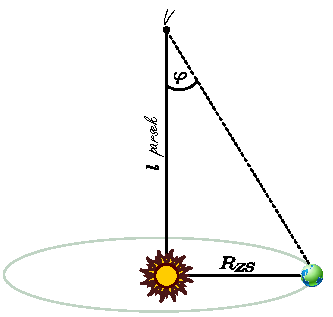
\includegraphics[width=0.6\linewidth]{fyz_fig224.pdf}
    \captionof{figure}[Parsek]{K příkladu \ref{FYZ:exam005}: Odvození velikosti Parseku}
    \label{fyz:fig224}
    \par}
  \begin{equation*}
    \varphi = \frac{R_{SZ}}{l} \rightarrow l = \frac{R_{SZ}}{\varphi},
  \end{equation*}
  kde $l$ je vzdálenost \SI{1}{\parsec} v metrech, $R_{SZ}$ je vzdálenost země od Slunce a 
  $\varphi$ je úhel jedné vteřiny vyjádřený v radiánech. 
  \begin{equation*}
      l = \frac{\SI{1.5e11}{\meter}}{\dfrac{1}{60\cdot60} 
          \cdot\dfrac{2\pi}{360}}\cong \SI{3e16}{\meter}.
  \end{equation*}
\end{example}
\wikitextrule
      %---------------------------------------------------------------
      Další jednotkou, kterou se v astrofyzice měří vzdálenost dvou vesmírných těles, je 
      \emph{paralaxa}. Pozorovací místa musí být od sebe výrazně vzdálena, aby například při měření 
      vzdálenosti naší nejbližší hvězdy - \emph{Proxima Centauri} byla paralaxa vůbec měřitelná. 
      Vzdálenost této hvězdy je \num{4.2} světelných let (nebo \SI{270000}{\AU}) od Země.
        
      %---------------------------------------------------------------
      % !TeX spellcheck = cs_CZ
\wikitextrule
\begin{example}\label{FYZ:exam006}
  Najděte paralaxu Proximy Centauri, která je od nás vzdálená asi \num{4.2} světelného roku 
  \protect\cite[s.~4]{Kulhanek2009}.
  
   {\centering
    \captionsetup{type=figure}
    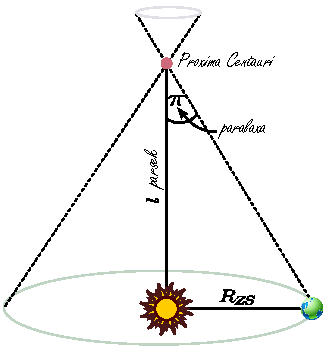
\includegraphics[width=0.8\linewidth]{fyz_fig225.pdf}
    \captionof{figure}{K příkladu \ref{FYZ:exam006}: Paralaxa naší nejbližší hvězdy}
    \label{fyz:fig225}
    \par}
    
  \textbf{Řešení}: Díky pohybu Země kolem Slunce se zdá, že blízké hvězdy opisují oproti 
  vzdáleným elipsu. Úhlový poloměr této elipsy se nazývá paralaxa hvězdy. Lze ji změřit jen pro 
  nejbližší hvězdy. Z definice úhlu (jako v předchozím příkladě) tedy vyplývá, že
  \begin{equation*}
    \pi = \frac{R_{ZS}}{l} = \frac{\SI{1.5e11}{\meter}}{\SI{4.2}{\lightyear}} 
        = \frac{\SI{1.5e11}{\meter}}{\num{4,2}\cdot\SI{9.5e15}{\meter}}
          \cong \SI{3,7e-6}{\radian},
  \end{equation*}
  
  což je přibližně \(\ang{;;0,76}\). Vidíme, že i u druhé nejbližší hvězdy po Slunci není 
  paralaxa ani celá \(\ang{;;1}\).
\end{example}
\wikitextrule
      %---------------------------------------------------------------
    
%} %tikzset
%---------------------------------------------------------------------------------------------------